\documentclass[italian]{beamer}

\hypersetup{unicode=true,
	%bookmarks=true,
	bookmarksnumbered=false,
	bookmarksopen=false,
	breaklinks=false,
	pdfborder={0 0 0},
	%backref=false,
	colorlinks=false,
	pdfpagemode=FullScreen,
	pdfauthor={Gionata Massi},
	pdfsubject={Presentazione della prova orale del concorso docenti 2016, classe di concorso A41 Scienze e tecnologie informatiche, di Gionata Massi.},
	pdfkeywords={Concorso docenti, A41, Informatica.}%
}

\usepackage[T1]{fontenc}
\usepackage[latin1]{inputenc}
\usepackage{babel}
%\usepackage{pgfpages}
%\usepackage{standalone}
\usepackage{verse}
\usepackage{booktabs}
\usepackage{multirow}
\usepackage{bookmark}
\usepackage{graphicx}
%\usepackage{eurosym}
%\usepackage{pgfplots}
%\usepgfplotslibrary{dateplot}     
\usepackage{tikz}
\usetikzlibrary{shapes}
\newcommand*\circled[1]{\tikz[baseline=(char.base)]{%
		\node[shape=ellipse,draw,inner sep=2pt] (char) {#1};}}

%\usepackage[]{algorithm2e}
%\usepackage{xmpmulti}

\usepackage{calc}
\usepackage[font=Times,timeinterval=59, timeduration=45.0, timedeath=1, fillcolorwarningsecond=white!60!yellow,
timewarningfirst=78,timewarningsecond=95]{tdclock}


\pgfdeclareimage[height=5mm]{CONCORSO}{img/banner_concorso_docenti}
\logo{\pgfuseimage{CONCORSO}}

\newcommand{\blu}[1]{{\usebeamercolor[fg]{structure} #1}}
\newcommand{\red}[1]{{\usebeamercolor[fg]{alerted text} #1}}



\setbeamertemplate{navigation symbols}{}
%\setbeamertemplate{frametitle continuation}[from second][(cont'd)]
\usefonttheme[stillsansseriftext,stillsansserifsmall]{serif}

\makeatletter

\mode<beamer|trans>{%
	\useoutertheme[glossy]{wuerzburg}
	\useinnertheme[shadow,outline]{chamfered}
	\usecolortheme{shark}
}


%% Save up on ink for the 4-up handouts
\mode<handout>{%
	\useoutertheme{wuerzburg}
	\useinnertheme[outline]{chamfered}
	%\pgfpagesuselayout{4 on 1}[a4paper, landscape, border shrink=10mm]
	\pgfpagesuselayout{2 on 1}[a4paper, portrait, border shrink=10mm]
	\pgfpageslogicalpageoptions{1}{border code=\pgfstroke}
	\pgfpageslogicalpageoptions{2}{border code=\pgfstroke}
	%\pgfpageslogicalpageoptions{3}{border code=\pgfstroke}
	%\pgfpageslogicalpageoptions{4}{border code=\pgfstroke}
}

\mode<presentation>{%
	\AtBeginSection{%
		\begin{frame}
			\frametitle{In questa sezione\ldots}
			\tableofcontents[ %
			currentsection,%
			hideothersubsections,%
			sectionstyle=show/hide,% 
			subsectionstyle=show/hide%
			]
		\end{frame}
	}
}
		
\title[Concorso docenti CdC A41]
{\Large{Processo di risoluzione degli indirizzi a livello applicativo}}

\institute[I.T.A. ``E. Sereni'']
{%
	{\scriptsize
Concorso personale docente\\
DD.DD.GG. n. 105, 106 e 107 del 23 febbraio 2016\\
Classe di concorso A41 -- Scienze e tecnologie informatiche}
}

\date[Roma, 21/07/2016 {\usebeamercolor[fg]{frametitle}\textbar}~\cronominutes]{Roma -- 21 Luglio 2016}

\newcommand\mybullet{\leavevmode%
\blu{\usebeamertemplate{itemize item}}\hspace{.5em}}

\begin{document}

\author[G. Massi]{%
	Ing. \textit{Gionata \textsc{Massi}}, PhD
}

\frame{\maketitle\initclock}
% \beamerdefaultoverlayspecification{<+->}
% \setbeamercovered{dynamic}

%\section*{Piano della presentazione}
%\subsection{Parte I: Esposizione di un percorso didattico}
\newcommand\boxednumber[1]
{%
	\hbox{%
		\usebeamerfont*{item projected}%
		\usebeamercolor[bg]{item projected}%
		\vrule width2.25ex height1.85ex depth.4ex%
		\hskip-2.25ex%
		\hbox to2.25ex{%
			\hfil%
			\color{fg}#1%
			\hfil}%
	}%
}

\begin{frame}{Piano della presentazione}
	\boxednumber{1} Parte~~~I: Illustrazione delle scelte contenutistiche, didattiche e metodologiche
	
	\medskip
	
	\boxednumber{2} Parte~~II: Esposizione di una lezione simulata
	
	\medskip
	\boxednumber{3} Parte~III: Interlocuzioni con il candidato
	\note{%
		{\tiny
			Buon pomeriggio,
			
			sono Gionata Massi e presenter\`o un percorso didattico sulla traccia estratta, riassunta dal titolo \dots.
			In 35 minuti dovrei illustrarvi la progettazione del percorso didattico, ipotizzando
			di avere di fronte una classe tipo e risorse didattiche infinite.
			
		}%tiny
	}%note
\end{frame}

\frame{
	\frametitle{Piano della presentazione del percorso didattico}
	\tableofcontents[part=1]
	\note{%
		{\tiny
			Buon pomeriggio,
			
			sono Gionata Massi e presenter\`o un percorso didattico sul \dots.
			
		}%tiny
	}%note
}

\frame{
	\frametitle{Piano della lezione}
	\tableofcontents[part=2]
	}

\frame{
	\frametitle{Piano del colloquio}
	\begin{center}\Huge{Any questions?}\end{center}
	}

\part[Percorso didattico]{Esposizione di un percorso didattico}
\frame{\partpage}

\section[Contesto]{Il contesto - traccia e ipotesi}

\begin{frame}{Traccia estratta}{Estratto}

	\begin{block}{\ldots{}il candidato analizzi il seguente caso concreto:}
		\large{processo di risoluzione degli indirizzi a livello applicativo}
	\end{block}
	
	\begin{block}{Su cosa devo preparare una lezione?}
		\begin{itemize}
			\item Lezione partecipata sul \alert{Domain Name System (DNS)} con IPv4.
			\item Attivit\`a di laboratorio usando \alert{\texttt{nslookup}} e \alert{\texttt{wireshark}}.
			\uncover<2>{\item In un tempo maggiore avrei potuto progettare le attivit\`a di laboratorio per la configurazione di \texttt{bind} su una rete di calcolatori emulata.}
		\end{itemize}
	\end{block}

\end{frame}

\begin{frame}{Scelta dell'istituto, della classe e della disciplina}{ITT -- I\&T -- Informatica -- classe $4^{\text{ta}}$ -- Sistemi e reti}
	
	\begin{block}{Istituto, settore, indirizzo, articolazione, disciplina}
		\noindent\mybullet Istituto \alert{Tecnico}
		
		\noindent\hspace*{0.5cm}\mybullet Settore \alert{Tecnologico}
		
		\noindent\hspace*{1.0cm}\mybullet Indirizzo \alert{Informatica e Telecomunicazioni}
		
		\noindent\hspace*{1.5cm}\mybullet Articolazione \alert{Informatica}
		
		\noindent\hspace*{2.0cm}\mybullet Disciplina \alert{Sistemi e reti}
	\end{block}
	
	\begin{block}{Territorio}
	\begin{itemize}
		\item Regione Marche
		\begin{itemize}
			\item PMI, pi\`u piccole che medie
			\item sviluppo di applicazioni gestionali
			\item settore telecomunicazioni e radar
			\item sistemi di misura e controllo
		\end{itemize}	
	\end{itemize}
	\end{block}
\end{frame}
	
\begin{frame}{Ipotesi della classe e situazione iniziale}{ITT -- I\&T -- Informatica -- classe $4^{\text{ta}}$ -- Sistemi e reti}
	
	\begin{block}{Classe}
		\begin{itemize}
			\item Classe $4^{\text{ta}}$
			\begin{itemize}
				\item 132 ore annue $\approx$ 4 ore a settimana
				\item di cui 2 in compresenza con l'insegnante tecnico pratico
				\item stimo circa 2$\frac{1}{2}$ ore settimanali di studio autonomo
			\end{itemize}			
			\item 20 alunni (18M / 2F)
			\item 0 alunni ripetenti
			\item 1 alunno BES disgrafico con PDP 
			\item la maggioranza degli alunni ha raggiunto un livello medio/alto
			\item tutte le lezioni sono in laboratorio, con una postazione PC connessa ad internet per ogni alunno
			\item il laboratorio \`e dotato di proiettore e lavagna bianca
		\end{itemize}
	\end{block}
	
\end{frame}

\section[Progettazione didattica]{Progettazione didattica}

\begin{frame}[allowframebreaks]{Quadro normativo}
%{Le leggi, le linee guida, le direttive ministeriali}
{Linee guida e direttive ministeriali}

	\begin{block}{d.P.R. n. 88 del 15 marzo 2010, articolo 8, comma 3 -- All. A.2}
		\noindent {\color{blue!50!black}``ISTITUTI TECNICI -- LINEE GUIDA PER IL PASSAGGIO AL NUOVO ORDINAMENTO''}
		% http://hubmiur.pubblica.istruzione.it/alfresco/d/d/workspace/SpacesStore/fd8ad76e-0e72-4ff2-aeff-0264b98168c3/linee_guida_tec_doc_completo_15_07_2010.pdf#page=63
		\medbreak
		\noindent\textbf{Presentazione sintetica ITT -- I\&T, estratto della pagina 63}
		\medbreak
		\mybullet L'indirizzo ``Informatica e Telecomunicazioni'' integra \alert{competenze} scientifiche e \alert{tecnologiche nel campo} dei sistemi informatici, dell'elaborazione delle informazioni, delle applicazioni e tecnologie Web, \alert{delle reti} e degli apparati \alert{di comunicazione}; \textit{omissis}
	\end{block}
	
	\begin{block}{Direttiva n. 4  del 16 gennaio 2012}
		\noindent {\color{blue!50!black} \textbf{in materia di Linee Guida per il secondo biennio e quinto anno per i percorsi degli Istituti Tecnici a norma dell'articolo 8, comma 3 del d.P.R. del 15 marzo 2010, n. 88.}}
		\medbreak
		Definisce, negli allegati, le schede disciplinari per il secondo biennio e quinto anno.
		\medbreak
		Allegato C4, ``ISTITUTI TECNICI -- LINEE GUIDA PER IL PASSAGGIO AL NUOVO ORDINAMENTO -- Schede disciplinari Secondo biennio e quinto anno''
		%http://banner.orizzontescuola.it/B1_AFM.pdf#page=3
	\end{block}\label{dir:16012012}
\end{frame}

\begin{frame}{Indicazioni ministeriali I}{Schede disciplinari -- Indirizzo ``Informatica'' -- ``Sistemi e Reti'', estratti All. C4}
		\begin{tabular}{p{\dimexpr \linewidth-2\tabcolsep}}
		\toprule
		\multicolumn{1}{c}{\bf Risultati di apprendimento del secondo biennio e quinto anno}\\
		\midrule
			\mybullet \alert{configurare, installare e gestire sistemi di elaborazione dati e reti}\\
			\mybullet scegliere dispositivi e strumenti in base alle loro caratteristiche funzionali\\
			\mybullet \alert{utilizzare le reti e gli strumenti informatici} nelle attivit\`a di studio, ricerca e approfondimento disciplinare\\
			\mybullet \alert{analizzare il valore, i limiti e i rischi delle varie soluzioni tecniche} per la vita sociale e culturale con particolare attenzione alla sicurezza nei luoghi di vita e di lavoro, alla tutela della persona, dell'ambiente e del territorio\\
		\bottomrule
		\end{tabular}
\end{frame}

\begin{frame}{Indicazioni ministeriali II}{Schede disciplinari -- Indirizzo ``Informatica'' -- ``Sistemi e Reti'', estratti All. C4}
		
		\centering
		\begin{tabular}{p{0.49\dimexpr \linewidth-2\tabcolsep}p{0.49\dimexpr \linewidth-2\tabcolsep}}
		\toprule
		\multicolumn{2}{c}{\bf Secondo biennio}\\
		\multicolumn{1}{c}{\bf Conoscenze} & \multicolumn{1}{c}{\bf Abilit\`a}\\
		\midrule
			\mybullet \alert{Organizzazione del software di rete in livelli} & \mybullet Individuare la corretta \alert{configurazione di una data applicazione}\\
			\mybullet Tipologie  e \alert{tecnologie delle reti locali e geografiche} & \mybullet Progettare, realizzare, configurare e gestire una rete\\
			\mybullet \alert{Protocolli per la comunicazione in rete}\\
			\mybullet \alert{Tecniche di gestione dell'indirizzamento di rete}\\
			\mybullet \alert{Problematiche di instradamento nelle reti geografiche}\\
			\mybullet \alert{Lessico e terminologia tecnica di settore} anche in lingua inglese & \mybullet \alert{Utilizzare il lessico e la terminologia tecnica di settore} anche in lingua inglese\\
		\bottomrule
		\end{tabular}
		
	\note{%

	}%note	
\end{frame}

%\begin{frame}{Programmazione didattica}{Quadro normativo delle attivit\`a funzionali all'insegnamento}
%	\begin{block}{CCNL Scuola 2006/2009 art. 29}
		
%		1. L'attivit\`a funzionale all'insegnamento {[}\ldots{]} comprende
%		tutte le attivit\`a, anche a carattere collegiale, di programmazione, progettazione,
%		ricerca, valutazione, documentazione, aggiornamento e formazione {[}\ldots{]}
		
%		\medskip
		
%		2. Tra gli adempimenti individuali dovuti rientrano le attivit\`a relative: 
		
%		\hspace*{0.5cm}a) alla preparazione delle lezioni e delle esercitazioni;
		
%	\end{block}
%\end{frame}

%\begin{frame}[allowframebreaks]{Definizioni}{Quadro europeo delle qualifiche}
%	\begin{description}
%		\item[risultati dell'apprendimento] descrizione di ci\`o
%		che un discente conosce, capisce ed \`e in grado di
%		realizzare al termine di un processo d'apprendimento.
%		I risultati sono definiti in termini di conoscenze,
%		abilit\`a e competenze;
		
%		\item[conoscenze] risultato dell'assimilazione di
%		informazioni attraverso l'apprendimento. Le
%		conoscenze sono un insieme di fatti, principi, teorie
%		e pratiche relative ad un settore di lavoro o di studio.
%		Nel contesto del Quadro europeo delle qualifiche
%		le conoscenze sono descritte come teoriche e/o
%		pratiche;
		
%		\item[abilit\`a] indicano le capacit\`a di applicare
%		conoscenze e di utilizzare know-how per portare a
%		termine compiti e risolvere problemi. Nel contesto
%		del Quadro europeo delle qualifiche le abilit\`a sono
%		descritte come cognitive (comprendenti l'uso del
%		pensiero logico, intuitivo e creativo) o pratiche
%		(comprendenti l'abilit\`a manuale e l'uso di metodi,
%		materiali, strumenti);
		
%		\item[competenze] comprovata capacit\`a di utilizzare
%		conoscenze, abilit\`a e capacit\`a personali, sociali
%		e/o metodologiche, in situazioni di lavoro o di
%		studio e nello sviluppo professionale e personale.
%		Nel contesto del Quadro europeo delle qualifiche
%		le competenze sono descritte in termini di
%		responsabilit\`a e autonomia.
%	\end{description}
%\end{frame}

\begin{frame}{Progettazione didattica}{Chi se ne occupa e in che modo. Ed io che progetto?}

\mybullet Il \alert{Dipartimento d'Informatica} stabilisce una pianificazione di massima identificando, per ogni anno di corso, i moduli didattici da realizzare. Essi sono progettati secondo le richieste del territorio e dell'Istituto, come espresso nel P(T)OF.

\mybullet Ogni modulo indica i prerequisiti, i risultati d'apprendimento (espressi in termini di competenze, conoscenze e abilit\`a), la collocazione e la durata temporale, i metodi e i materiali didattici, la tipologia e il numero minimo di verifiche, eventualmente comuni per classi parallele.

\mybullet Il docente pu\`o integrare la programmazione, di concerto con il consiglio di classe, con UdA e compiti autentici per la certificazione di competenze trasversali.

\mybullet La parte seguente \`e la mia progettazione di un ciclo di lezioni nel modulo sul livello di applicazione, che segue quelli sui livelli di rete e trasporto, limitatamente al ``Domain Name System''.

\end{frame}

\begin{frame}[allowframebreaks]{Prerequisiti, conoscenze pregresse, motivazioni}{Per la programmazione e la riprogettazione dell'attivit\`a didattica}

%	Non si pu\`o programmare un'attivit\`a didattica senza conoscere la classe.
	
%	Andrebbero lette le relazioni finali e verificate le conoscenze in ingresso!
	
	Assumeremo che i seguenti prerequisiti di conoscenza siano stati conseguiti (e certificati).
		
	\begin{block}{Prerequisiti e conoscenze pregresse}
		I concetti base e gli aspetti implementativi dei protocolli delle applicazioni di rete
		
		\begin{itemize}
			\item la commutazione di pacchetto, i protocolli IP e TCP;
			\item i modelli di servizio del livello di trasporto (livello 4 del modello ISO/OSI);
			\item i modelli di servizio del livello di rete (livello 3 del modello ISO/OSI);
			\item il paradigma client-server;
			\item la composizione di una URL.
		\end{itemize}
	\end{block}
	
	%\begin{block}{Conoscenze pregresse che l'insegnante pu\`o sondare}
	%	Gli studenti hanno gi\`a esperienza d'uso del Web e di altre applicazioni di rete realizzate con le tecnologie del Web.
		
	%	\medskip
		
	%	I ``nativi digitali'' sono stati tenuti all'oscuro di quanto c'\`e dietro ad un software. Questo \`e materia di sondaggio per la progettazione dell'attivit\`a didattica e di motivazione.
	%\end{block}
	
	%\framebreak
	
	%\framebreak

	%\begin{block}{Esperienze pregresse}
	%	Scambiare informazioni/comunicare tra esseri umani
	%	\begin{itemize}
	%		\item \textbf{blog};
	%		\item \textbf{forum}
	%		\item \textbf{social network}
	%		\item \textbf{wiki};
	%		\item \textbf{giochi online}
	%	\end{itemize}
		
	%	Soddisfare esigenze specifiche con web application
	%	\begin{itemize}
	%		\item \textbf{commercio elettronico}
	%		\item \textbf{mappe} e \textbf{ricerca di percorsi} in un grafo stradale
	%		\item \textbf{web-mail}
	%		\item \textbf{calendari} e \textbf{strumenti collaborativi}
	%	\end{itemize}
	%\end{block}
		
	\begin{block}{Motivare allo studio: fare leva sui bisogni di}
		\begin{description}
			\item[autostima] stima da parte dei compagni e degli insegnanti\\\hfill\textbf{peer assessment}
			\item[auto-efficacia] apportare il proprio contributo\\\hfill\textbf{peer assessment, mini-progetto}
			\item[potere] dominare la realt\`a\\\hfill\textbf{(ri)conoscere architetture e tecnologie della rete}
			\item[avere uno scopo] dare un senso alle nozioni apprese\\\hfill\textbf{configurare bind, analizzare con uno sniffer, riconoscere minacce, mini-progetto}
			\item[sfida] difficolt\`a da superare\\\hfill\textbf{mini-progetto}
		\end{description}
	\end{block}
\end{frame}

\subsection[Finalit\`a]{Obiettivi generali}
\begin{frame}{Obiettivi generali}{Le finalit\`a del modulo didattico}
	Con riferimento alle competenze, alle conoscenze e alle abilit\`a definite dalla Direttiva n. 4 del 16/01/2012 in materie di Linee Guida per la classe prescelta \hyperlink{dir:16012012}{\beamerreturnbutton{estratto linee guida}}, si declina l'unit\`a didattica sul DNS allo scopo di sviluppare le competenze per:
	
	\begin{itemize}
		\item \alert{progettare, sviluppare e realizzare applicazioni distribuite e scalabili.}
	\end{itemize}
	
	\note{%
		
	}%note	
\end{frame}

\subsection[Obiettivi]{Obiettivi d'apprendimento}
\begin{frame}{Obiettivi come prestazioni misurabili}{DNS}
	
	% 		\item Comprendere quali sono i principali componenti architetturali di una ``web page'' moderna e le loro inter-connessioni.
	
	{\tiny
	\begin{table}
		\begin{tabular}{@{}p{0.2\textwidth}p{0.75\textwidth}@{}} \toprule
			\multicolumn{1}{c}{Abilit\`a} & \multicolumn{1}{c}{Obiettivo} \\ \midrule
			
			\multirow{3}{*}{\parbox{0.2\textwidth}{Comprendere ed utilizzare il linguaggio tecnico}}
			 & Elencare le componenti di un'applicazione di rete.\\
			 & Definire i flussi di dati ed elaborazioni nel caso di query DNS.\\
			 & Mettere in relazione richieste e risposte DNS.\\
			 & Definire i termini \textit{Domain Name System}, \textit{Uniform Resource Locator} (URL), \textit{Fully Qualified Domain Name} (FQDN), \textit{name server}.\\
			 
			 \\
			 
			 \multirow{3}{*}{\parbox{0.2\textwidth}{Impostare il nome di dominio e i name server}}
			 & Saper usare il comando \texttt{hostname}.\\
			 & Saper configurare il file \texttt{/etc/hosts}.\\
			 & Saper leggere e modificare il file \texttt{/etc/resolv.conf}.\\
			  \\
			 
			 
			 \multirow{2}{*}{\parbox{0.2\textwidth}{Interrogare un name server}}
			 & Visualizzare richieste e risposte DNS intercorse fra l'host e il name server.\\
			 & Visualizzare il name server di competenza.\\
			 
			 \\
			
			 \multirow{2}{*}{\parbox{0.2\textwidth}{Valutare le tecnologie}}
			 & Illustrare i vantaggi e gli svantaggi dell'erogazione del servizio DNS su protocollo UDP confrontandolo con il TCP.\\
			 & Saper confrontare il modello di servizio ricorsivo rispetto a quello iterativo.\\
			
		\bottomrule
		\end{tabular}
		\caption{Obiettivi}
	\end{table}
	}
	
\end{frame}

\subsection[Strategie\ldots]{Metodologie, strategie e strumenti didattici utilizzati}

\begin{frame}[fragile]{Un approccio laboratoriale}{Apprendimento guidato dall'esperimento}
	
	\begin{columns}
		\begin{column}{0.3\textwidth}
			
			\newcommand{\autore}[1]{%
				\nopagebreak{\raggedleft\footnotesize #1\par}}
				
			\settowidth{\versewidth}{Se ascolto dimentico,}
			{\color{green!50!black}	
			\begin{verse}[\versewidth]
			\begin{altverse}
				Se ascolto dimentico,\\
				Se vedo ricordo,\\
				Se faccio imparo\\
				\autore{Confucio}
			\end{altverse}
			\end{verse}
			}
			
			\vfill
			
			\begin{itemize}
				\item in laboratorio;
				\item col computer;
				\item tanti elaborati;
				\item peer assessment;
				\item mini-progetto.
			\end{itemize}
			
			Quali fasi?
						
		\end{column}
		
		\begin{column}{0.7\textwidth}
			
			\begin{enumerate}
				\item Elicitazione delle conoscenze pregresse sui nomi di dominio e sue tecnologie e motivazione con esempi derivanti esperienze;
				
				\item proposizione di problematiche, esposizione di strategie risolutive, sperimentazione al computer;
				
				\item prove formative in itinere con produzione di elaborati individuali (relazioni delle attivit\`a);
				
				\item prova sommativa, illustrazione della soluzione e peer assessment;
				
				\item mini-progetto con potenziamento e/o recupero.
			\end{enumerate}			
			
		\end{column}
	\end{columns}

	\note{%
		
	}%note	
\end{frame}

\subsection[Strumenti\ldots]{Software di ausilio alla didattica}
\begin{frame}{Strumenti per imparare facendo}{Con cosa esercitarsi}
	\begin{itemize}
		\item Linux box
		
		\item nslookup
		
		\item wireshark
		
		\item Il video ``\hyperlink{https://youtu.be/D-VCk4_GMjQ?list=PLa_solX20V8I8t5sIW7A5Vx3v5YZ-OM3S}{IP Address and DNS}'' di code.org
		
		\item Moodle per la gestione del corso
		
		\item Libro di testo consigliato:  Lo Russo \& Bianchi, ``Sistemi e Reti -- Volume 2'', Hoepli
		
		\item Kurose \& Ross, ``Internet e Reti di Calcolatori'', McGraw-Hill (potenziamento, slide)
		
		\item RFC 1034 e 1035 (potenziamento, miniprogetto)
		
		\item Giacomini, ``Appunti di informatica libera'', Capitolo 33. Risoluzione dei nomi. Disponibile online alla pagina \url{http://a2.pluto.it/a2/risoluzione_dei_nomi.htm}
		
	\end{itemize}
	\note{%
		
	}%note	
\end{frame}

\section[Modi e tempi]{Modi e tempi del segmento didattico}
\begin{frame}{Modi e tempi}{Pianificazione delle lezioni}
	
	\begin{block}{Quando?}
	Marzo, dopo i moduli sul livello di rete e di trasporto.
	\end{block}
	
	\begin{block}{Quanto? e in che modo?}
	\begin{itemize}
		\item 4 ore di lezione partecipata.
		\item 4 ore di attivit\`a di laboratorio
		\item 4 ore di lavoro autonomo per studio e valutazione peer-assessment.
	\end{itemize}
	\end{block}

	\begin{block}{Insieme a chi?}
		``\alert{Informatica}'' e ``\alert{Tecnologie e progettazione di sistemi informatici e telecomunicazioni}'' (database, ricorsione, sistemi operativi, caching, progettazione e realizzazione del codice). ``\alert{Inglese}'' (corretta pronuncia dei termini, lettura delle man page e delle RFC).
	\end{block}
%	\centering\includegraphics[trim={2cm 14.5cm 2cm 2cm},clip,width=0.95\textwidth]{img/gantt}		
\end{frame}


\section[Verifica e valutazione]{Verifica e valutazione}
\begin{frame}{Valutazione condivisa}{Valutazione per spingere al miglioramento}
	
	\begin{itemize}
		\item verifiche formative a casa, una dopo ogni lezione teorica, con quiz a risposta multipla
		\item peer assessment di 3 elaborati prodotti dai compagni di classe (double-blind)
		\item mini-progetto
	\end{itemize}
	
%	\centering\includegraphics[width=0.6\textwidth]{img/mini_progetto}
	\note{%
		
	}%note	
\end{frame}

\section[Adattamenti per BES]{Adattamenti per BES}
\begin{frame}{Strumenti compensativi e misure dispensative}{Per BES e DSA}
	
	Strumenti compensativi
	\begin{itemize}
		\item si usano gi\`a strumenti informatici ``compensativi''
		\item l'argomento non presenta livelli di astrazione elevati
	\end{itemize}
	
	Misure dispensative
	
	\begin{itemize}
		\item a seconda del caso:
		\begin{itemize}
			\item aumento del tempo della prova
			\item dispensa da esercizi pi\`u astratti
			\item programmazione per obiettivi minimi
			\item prove oggettive
			\item dispensa dal valutare altre prove
		\end{itemize}
	\end{itemize}
	
	Recupero individualizzato, in particolare durante le ore in compresenza.
			
	\note{%
		
	}%note	
\end{frame}

\part[Lezione simulata]{Esposizione della lezione}
\frame{\partpage}

\section[Il problema]{Il problema}

\begin{frame}{Il problema}{Ricordarsi i codici}

Dopo aver visto a casa  il video ``\hyperlink{https://youtu.be/D-VCk4_GMjQ?list=PLa_solX20V8I8t5sIW7A5Vx3v5YZ-OM3S}{IP Address and DNS}'' di code.org


\begin{exampleblock}{Codici e nomi}
\mybullet Per l'Agenzia delle Entrate sono il contribuente ``MSSGNT80A21H769K''.

\mybullet Per gli amici sono ``Gionata''. Il nome \`e sufficiente ad identificarmi in famiglia.
Ma non lo era all'universit\`a quando tra i miei compagni di corso avevo un omonimo. Per chiamarmi con la sicurezza di rifersi a me dovevano usare anche il cognome: ``Gionata Massi''.
\end{exampleblock}

\begin{block}{Domande}
\mybullet \`E pi\`u facile ricordare il nome o il codice fiscale?

\mybullet C'\`e un algoritmo per passare dal CF al nome? Come dobbiamo fare?
\end{block}

\end{frame}

\begin{frame}{Il problema}{Ricordarsi i 32 bit di un indirizzo IPv4}

\begin{exampleblock}{Indirizzi IP e nomi degli host}

\mybullet Un host \`e identificato da un indirizzo IP di 32 bit, per comodit\`a di lettura raggruppato in quattro gruppi da 8.


\mybullet Per ricordarci la sua funzione o dove si trova un host usiamo un nome (hostname) facile da ricordare per un essere umano. Per i limiti dei protocolli di rete occorre considerare che ci sono dei limiti sul numero di caratteri.

\mybullet Tanti host svolgono lo stesso compito, ad esempio servire pagine web. Potremmo chiamarlo \texttt{www}, ma come identificarlo tra tanti host che si chiamano cos\`i? I domini! 
\end{exampleblock}

\begin{block}{Domanda}
\mybullet Come realizzare una mappa tra i nomi dei computer e i loro indirizzi IP?

\mybullet Allora che significano i punti, ad esempio in \texttt{www.istruzione.it}?

\end{block}

\end{frame}

\begin{frame}{Il Domain Name System}{Definizione}

	\begin{block}{Definizione}
	   Con \alert{Domain Name System} (\alert{DNS}) si intende:
	   
		\mybullet un database distrubuito che memorizza coppie (nome host, indirizzo IP) di un insieme di host
		
		\mybullet un protocollo a livello di applicazione che regola la comunicazione tra host e name server
	\end{block}
\end{frame}


\begin{frame}{Il Domain Name System}{Funzionalit\`a}

	\begin{block}{Funzionalit\`a}
		\begin{enumerate}
			\item traduzione dei nomi simbolici in indirizzi
			\item gestione degli alias
			\item bilanciamento del carico -- nel caso di servizi offerti da pi\`u host
		\end{enumerate}
	\end{block}
\end{frame}

\section[La soluzione]{La soluzione}

\begin{frame}{Progettazione della soluzione}{Primo tentativo}

\begin{exampleblock}

\mybullet Il servizio \`e erogato da un unico host, che chiamiamo name server.

\mybullet Il name server esegue operazioni CRUD su una tabella che mantiene la coppia di valori (hostname, indirizzo IP). 

\end{exampleblock}

\begin{block}{Domande}

\mybullet Che succede se il name server non \`e raggiungibile?

\mybullet Si prevede la possibilit\`a di congestione della rete? O di negazione del servizio?

\mybullet I tempi di fruizione del servizio sono omogenei per tutti gli host della rete?

\mybullet Che succede se devo aggiungere/cancellare/modificare host?

\mybullet La soluzione centralizzata \`e scalabile?
\end{block}
\end{frame}

\begin{frame}{Progettazione della soluzione}{Come \'e progettato realmente il DNS I}

\begin{block}{Tanti database scalabili e vicini}

\mybullet Il database dei nomi degli host deve essere distribuito su pi\`u name server.

\mybullet Un organizzazione dei nomi gerarchica (dominio) consente di separare le responsabilit\`a dei name server.

\mybullet Un sistema di caching: dopo la prima richiesta le query non si propagano. \uncover<2>{\alert{Analogie con: tabelle di lookup e tecniche di programmazione tipo memoize, organizzazione della memoria\ldots{}}}
\end{block}
\end{frame}

\begin{frame}{Progettazione della soluzione}{Come \'e progettato realmente il DNS II}

\begin{block}{La struttura gerarchica}

	\mybullet Server di nomi radice (root DNS server)
	
	\mybullet Server top-level domain (TLD server)
	
	\mybullet Server di competenza (authoritative)
\end{block}
\end{frame}

\begin{frame}{Progettazione della soluzione}{Come \'e progettato realmente il DNS III}

\centering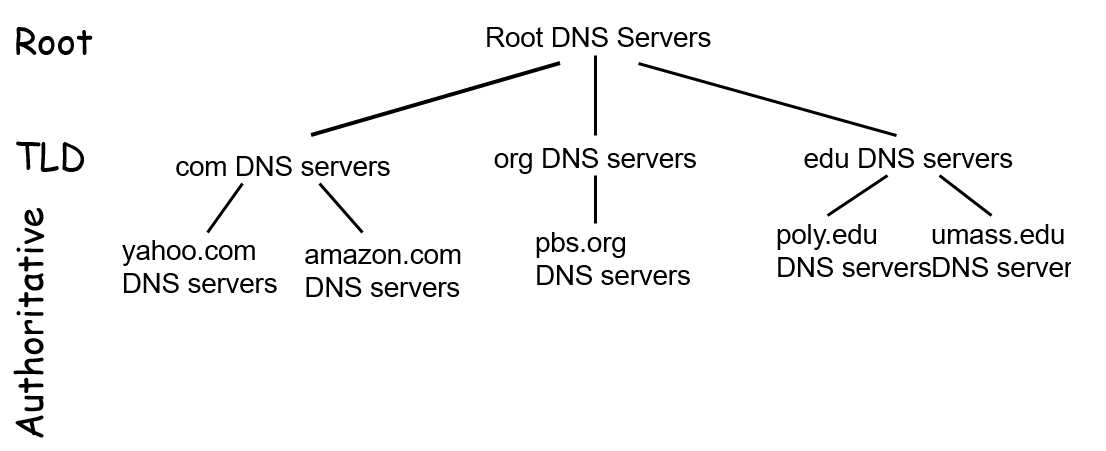
\includegraphics[width=\textwidth]{img/gerarchia}

\end{frame}


\begin{frame}{Progettazione della soluzione}{Come \'e progettato realmente il DNS III}

\centering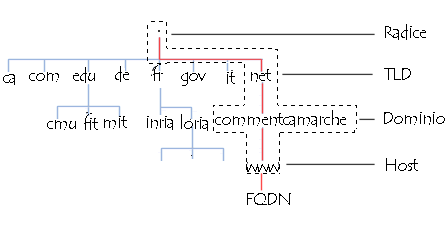
\includegraphics[width=\textwidth]{img/domini}

\end{frame}

\section[Realizzazione del servizio]{Realizzazione del servizio DNS}

\begin{frame}{Local name server}{Il mio DNS?}
\begin{block}
	
	\mybullet Non appartiene alla gerarchia
	
	\mybullet Ogni ISP ha un default name server
	
	\mybullet La query DNS di un host viene inviata al default name server, che si comporta come un proxy e, se non conosce il record da restituire, inoltra la richiesta ai livelli pi\`u alti della gerarchia
\end{block}

\begin{block}{Domande sui name server locali}
	
	\mybullet Dove lo leggo?
	
	\mybullet Quanti sono?
	
	\mybullet Come lo/i modifico?
	
	\mybullet Come mi viene/vengono assegnato/i? 
\end{block}
\end{frame}

\begin{frame}{Risoluzione dei nomi di dominio}{gethostbyname}
\begin{block}{Il resolver}
  \mybullet Il resolver \`e il processo (l'insieme di funzioni) che interroga gli Internet name server e ne interpreta le risposte.
  
  \mybullet la sua configurazione \`e memorizzata in \texttt{/etc/resolv.conf} e in \texttt{/etc/host.conf}
\end{block}

\begin{block}{Processo di risoluzione}
\begin{enumerate}
\item Il client interroga il DNS, chiedendo l'indirizzo per un dominio;
\item Il DNS restituisce il record;
\item Il client si connette all'indirizzo contenuto nel record.
\end{enumerate}
\end{block}
\end{frame}

%%%
\begin{frame}{Risoluzione dei nomi di dominio -- Recursive I}{Query ricorsiva}
\begin{block}{Processo di risoluzione nel caso ricorsivo}
\begin{enumerate}
\item Il client chiede al Local NS l'indirizzo del dominio;
\item Il Local NS delega la richiesta al Root NS;
\item Il Root NS delega la richiesta al TLD NS;
\item Il TLD NS interroga il NS autoritativo per il dominio;
\item Il NS autoritativo rimanda il record al TLD NS. Il record viene passato tra tutti i NS coinvolti, fino al Local NS;
\item Il Local NS restiruisce l'indirizzo al client, che raggiunge la destinazione.
I NS sono interrogati ricorsivamente. Ogni NS coinvolto, interroga il successivo, che interroger\`a quello successivo ancora.
\end{enumerate}
\end{block}
\end{frame}

\begin{frame}{Risoluzione dei nomi di dominio -- Recursive II}{Query ricorsiva}
\centering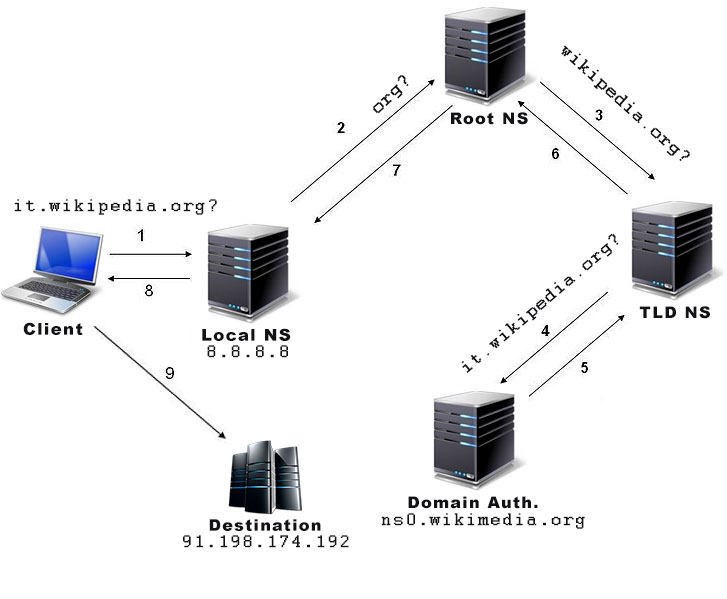
\includegraphics[height=0.8\textheight]{img/dns-risoluzione-ricorsiva}
\end{frame}

\begin{frame}{Risoluzione dei nomi di dominio -- Iterative I}{Query iterativa}
\begin{block}{Processo di risoluzione nel caso iterativo}
\begin{enumerate}
\item Il client chiede al Local NS l'indirizzo del dominio;
\item Il Local NS interroga il Root NS, per l'indirizzo del NS autoritativo per il TLD del dominio;
\item Il Local NS interroga il TLD NS, per l'indirizzo del NS autoritativo per il dominio richiesto;
\item Il Local NS interroga il NS autoritativo per il dominio, per l'indirizzo della risorsa richiesta;
\item Il Local NS restituisce l'indirizzo al client, che raggiunge la destinazione.
\end{enumerate}
\end{block}
\end{frame}

\begin{frame}{Risoluzione dei nomi di dominio -- Iterative II}{Query iterativa}
\centering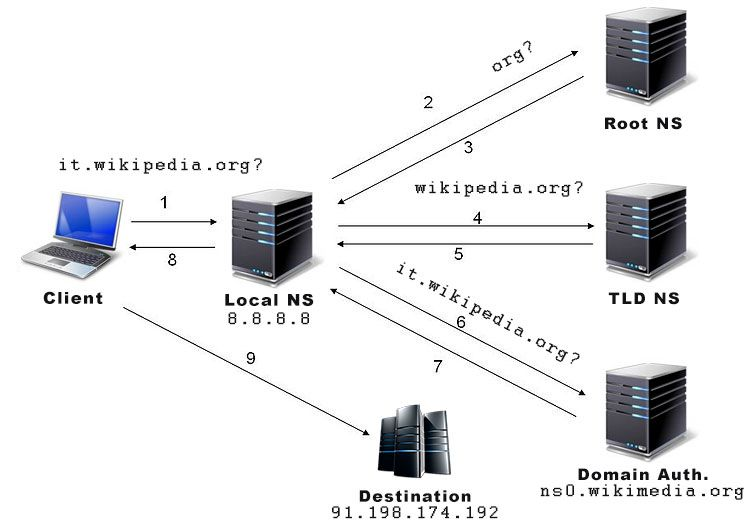
\includegraphics[height=0.8\textheight]{img/dns-risoluzione-iterativa}
\end{frame}
%%%
\section{Laboratorio}

\subsection[Lab 1: nslookup]{Query con \texttt{nslookup}}

\begin{frame}{Interrogare il DNS}{Usare \texttt{nslookup}}

\only<1,3,5,7>{
\begin{block}{Sfide -- usare \texttt{nslookup} in modo interattivo}
\begin{block}{Leggere insieme la pagina di manuale di \texttt{nslookup}}
\texttt{man nslookup}
\end{block}

Chiedere in modo interattivo l'indirizzo dell'host \texttt{ricop.dii.univpm.it}
\begin{enumerate}
	\item al name server predefinito 
	\item \uncover<3->{al name server 8.8.8.8}
	\item \uncover<5->{abilitando la visualizzazione completa del pacchetto di risposta}
	\item \uncover<7->{visualizzando le informazioni sull'host}
\end{enumerate}
\end{block}
}
\only<2>{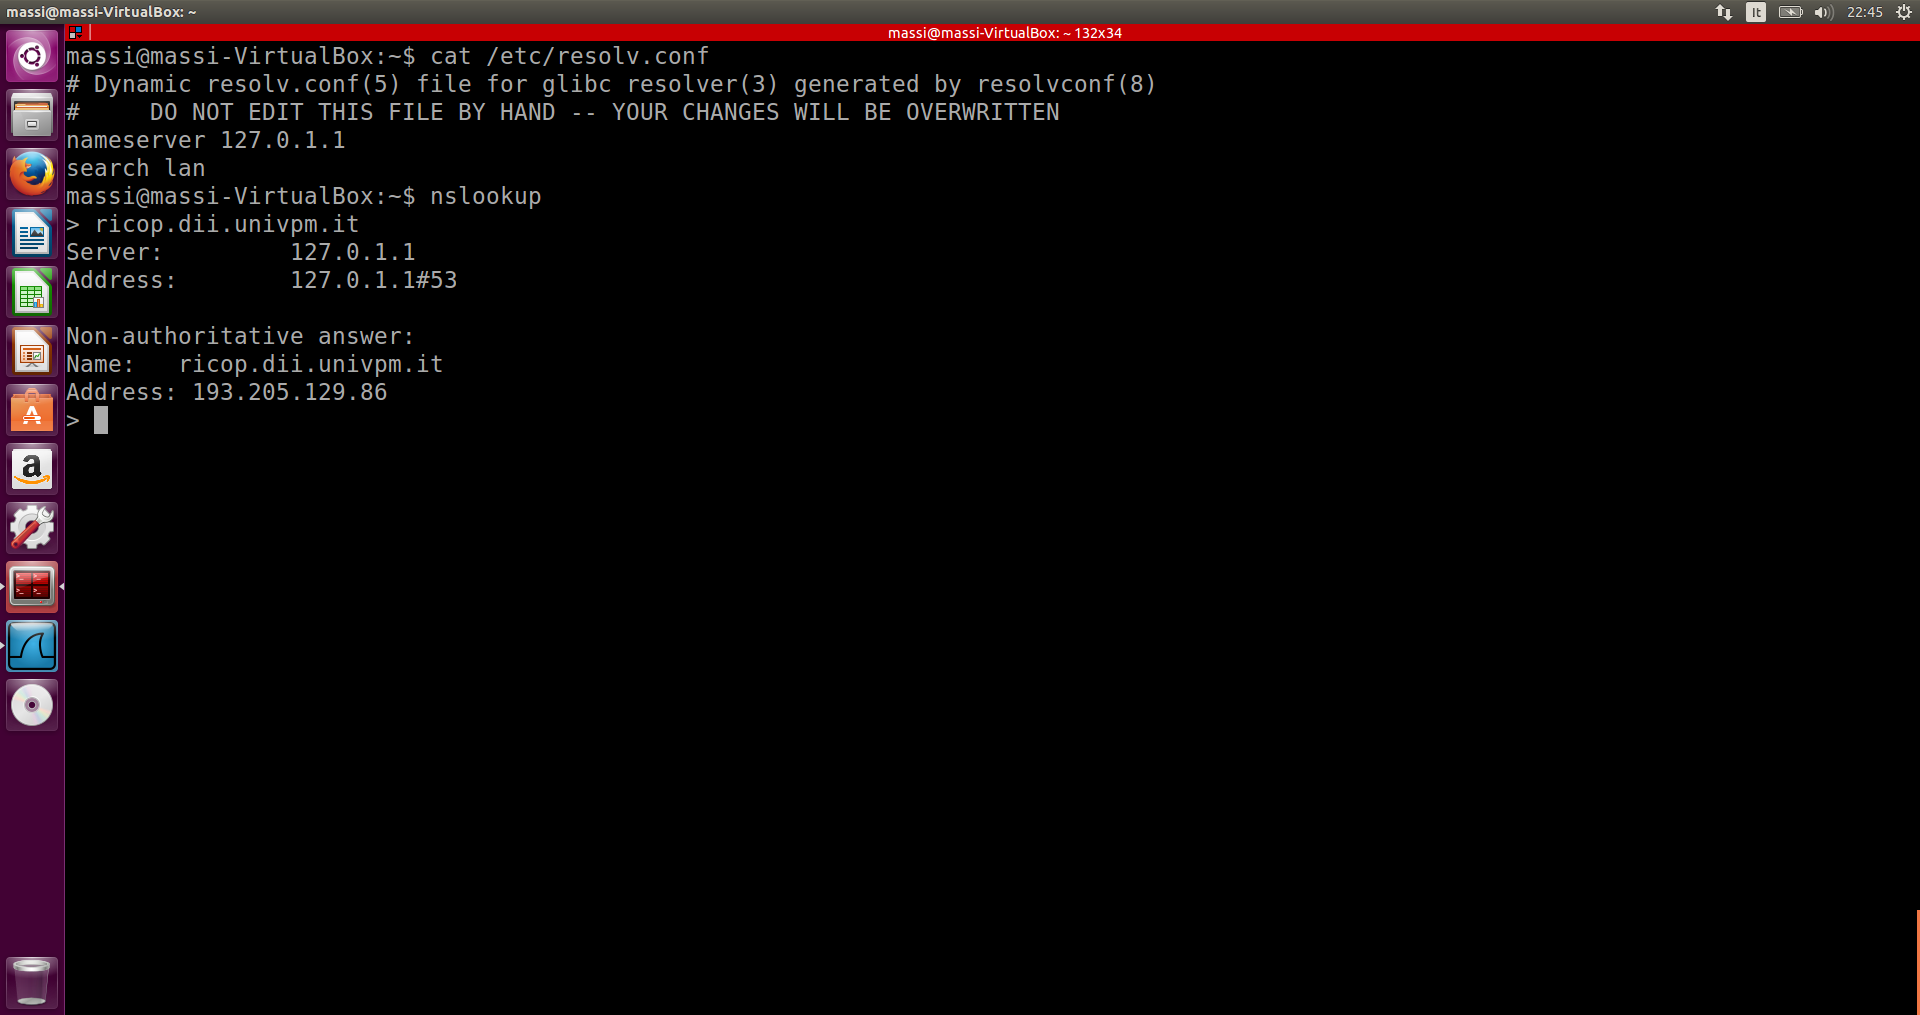
\includegraphics[width=\textwidth]{img/lab1_1}}
\only<4>{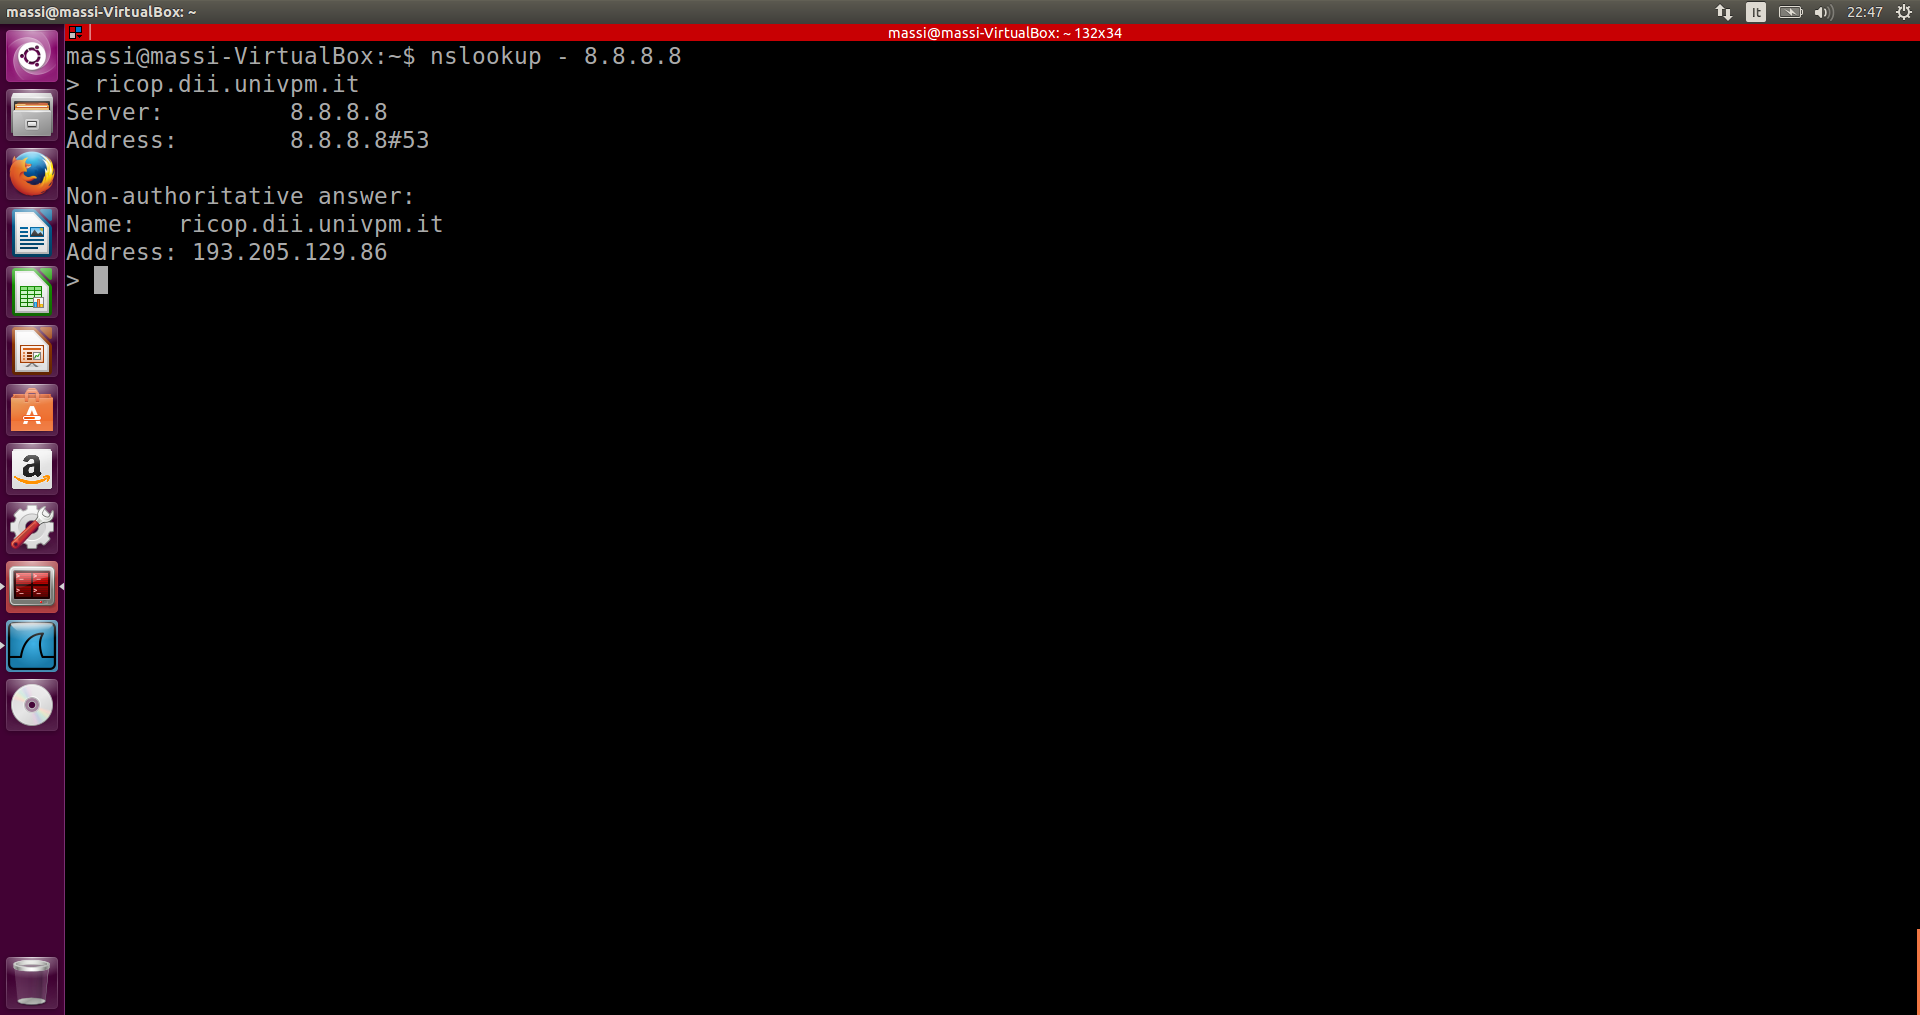
\includegraphics[width=\textwidth]{img/lab1_2}}
\only<6>{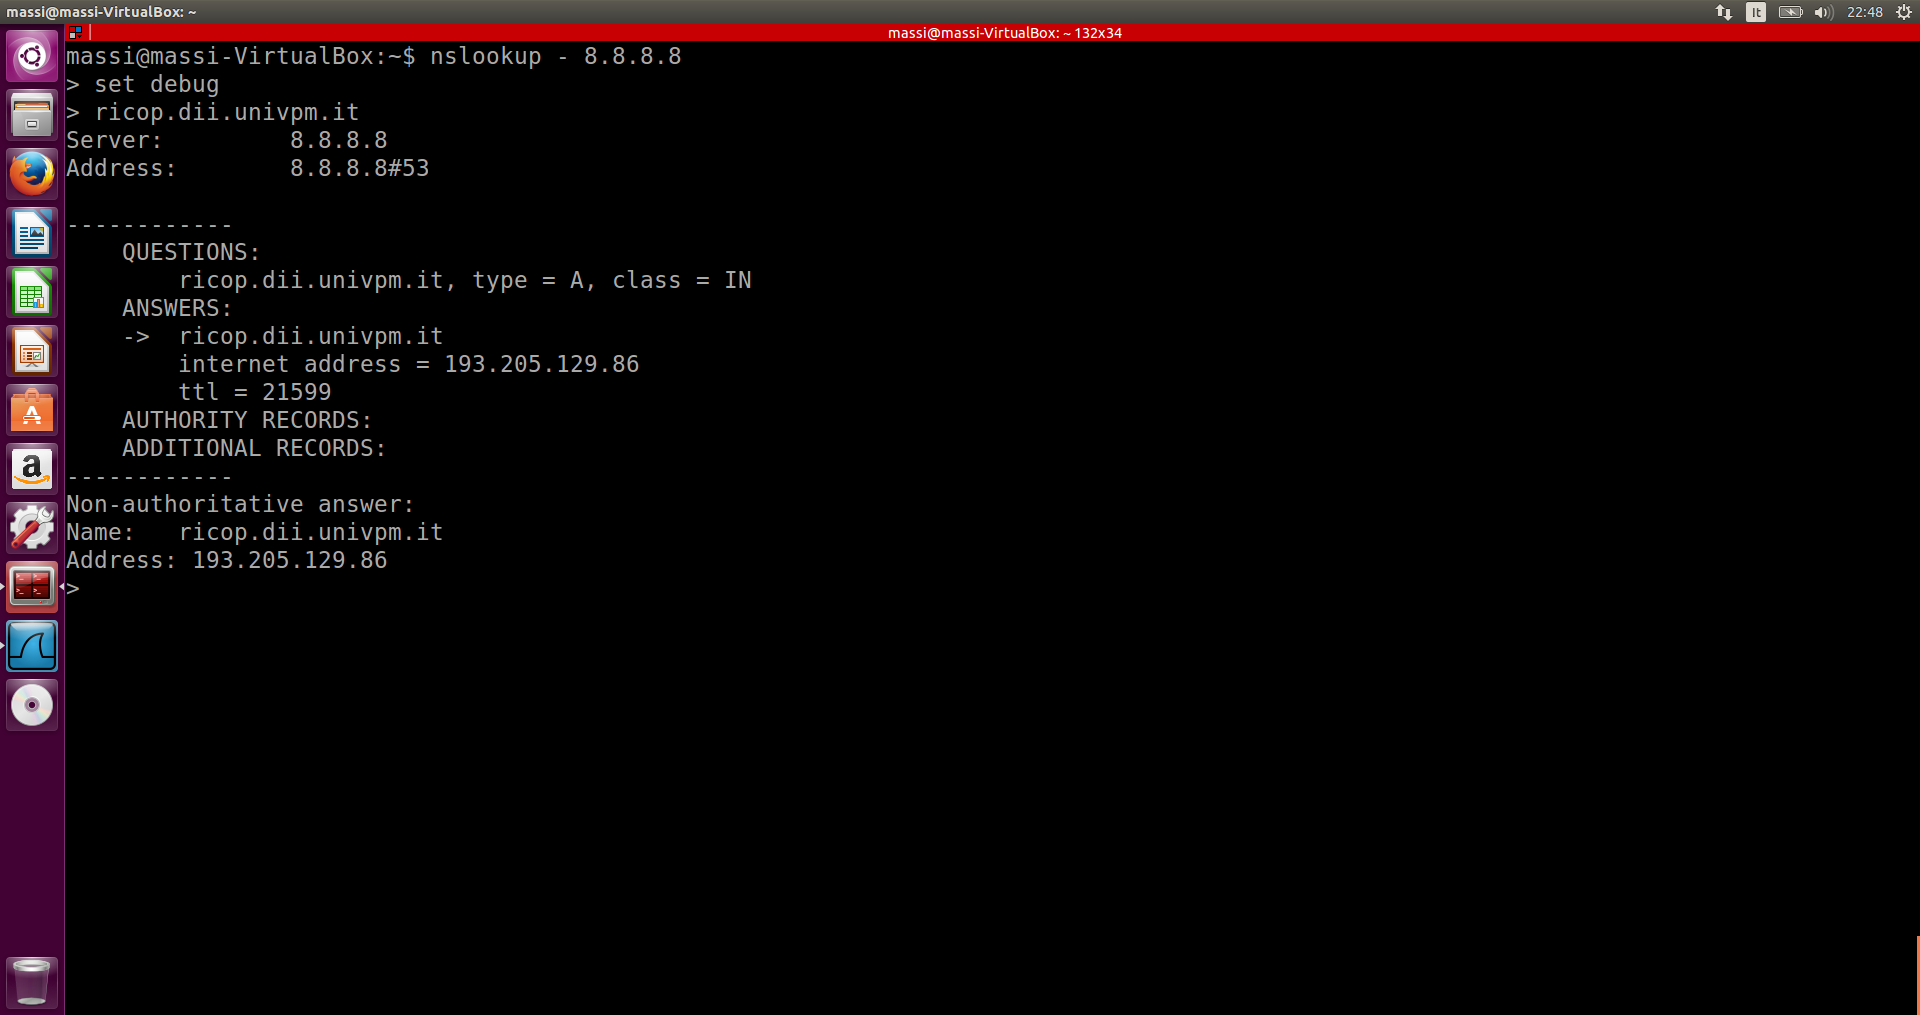
\includegraphics[width=\textwidth]{img/lab1_3}}
\only<8>{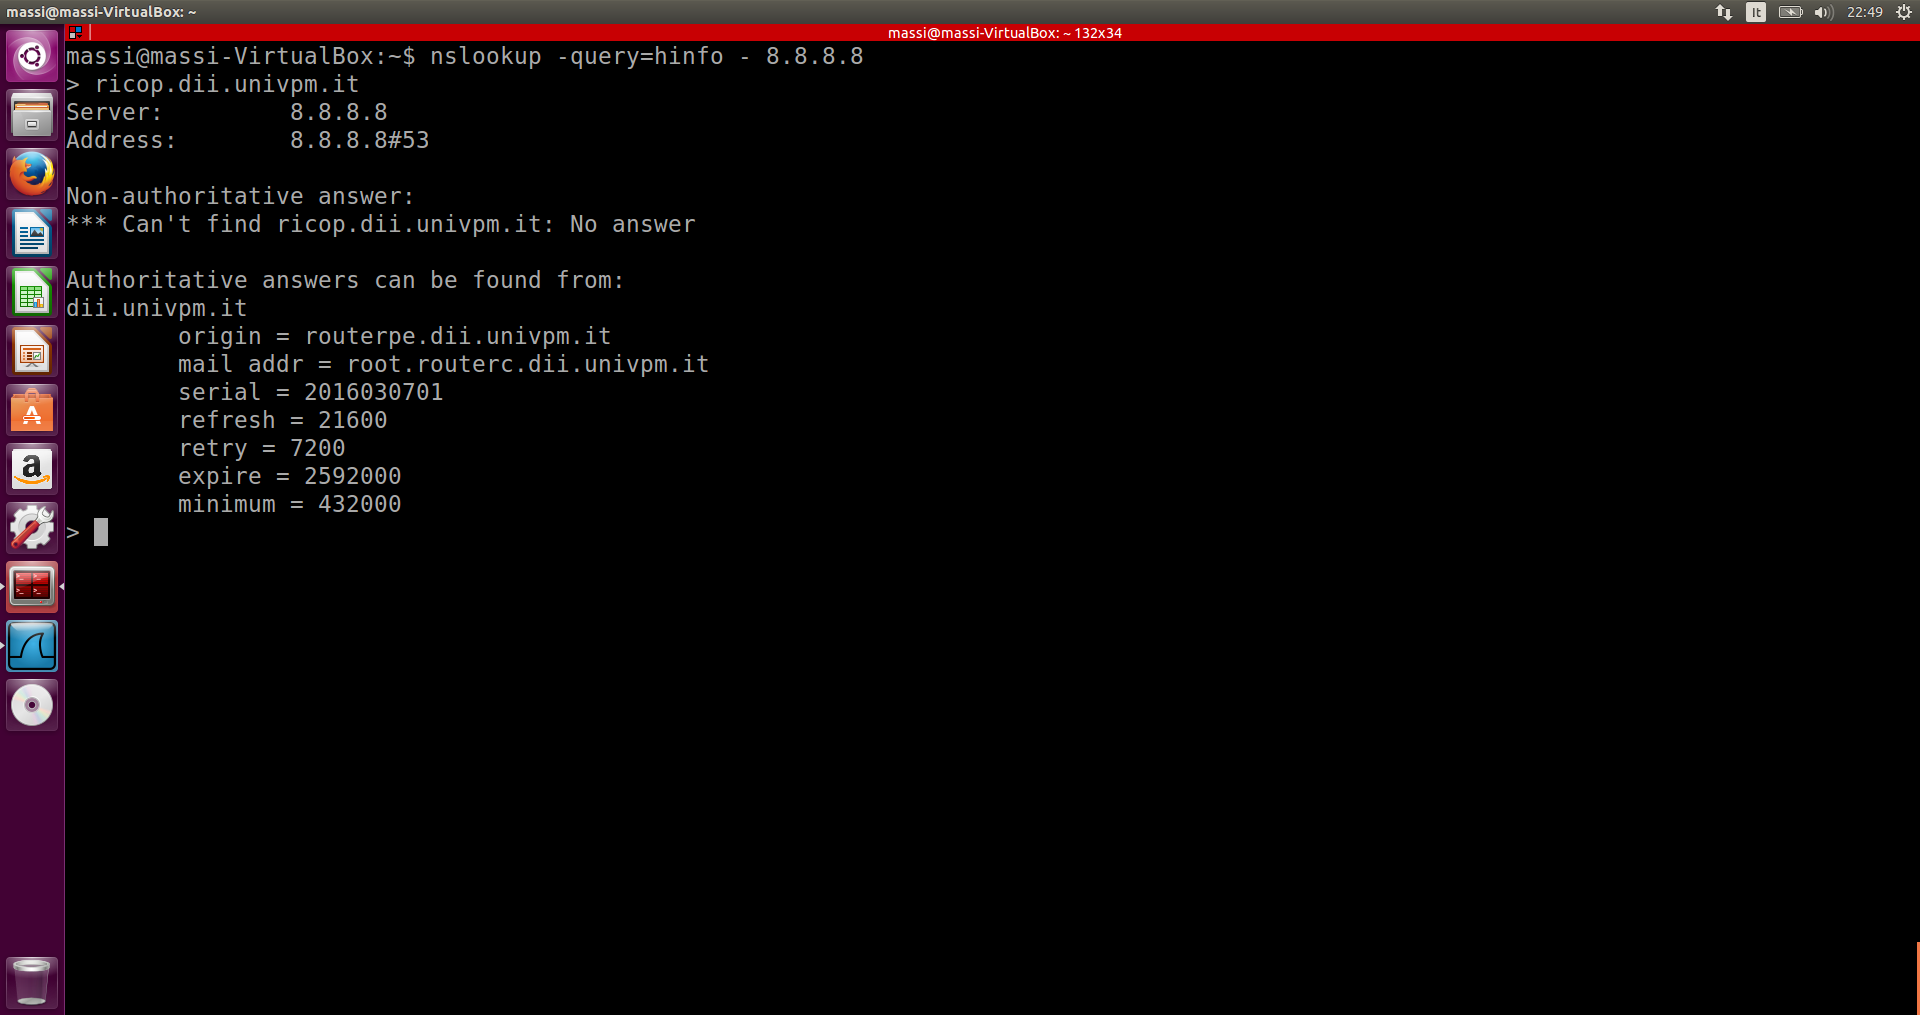
\includegraphics[width=\textwidth]{img/lab1_4}}

\end{frame}


\subsection[Lab 2: wireshark]{Analisi del protocollo DNS con \texttt{wireshark}}

\begin{frame}{Analisi del protocollo DNS}{Usare \texttt{wireshark}}
\only<1,3>{
\begin{block}{Sfide -- usare \texttt{wireshark} per visualizzare query DNS}

Wireshark e netcat (nc) li conosciamo dai moduli precedenti (rete e trasporto) e attuale (applicazione).

\begin{enumerate}
	\item Come filtrare la visualizzazione dei soli pacchetti DNS? Elencare almeno due modi!
	\item \uncover<3>{Mostrare i pacchetti del protocollo DNS catturati navigando il sito wikiricop.dii.univpm.it}
	\item \uncover<3>{Confrontare i record letti con nslookup e cattuari con wireshark}
	\item \uncover<3>{Forgiare una query DNS con \texttt{nc}, catturare la risposta con \texttt{wireshark} ed indicare l'indirizzo IP dell'host \texttt{www.google.com}}.
\end{enumerate}
\end{block}
}
\only<2>{\centering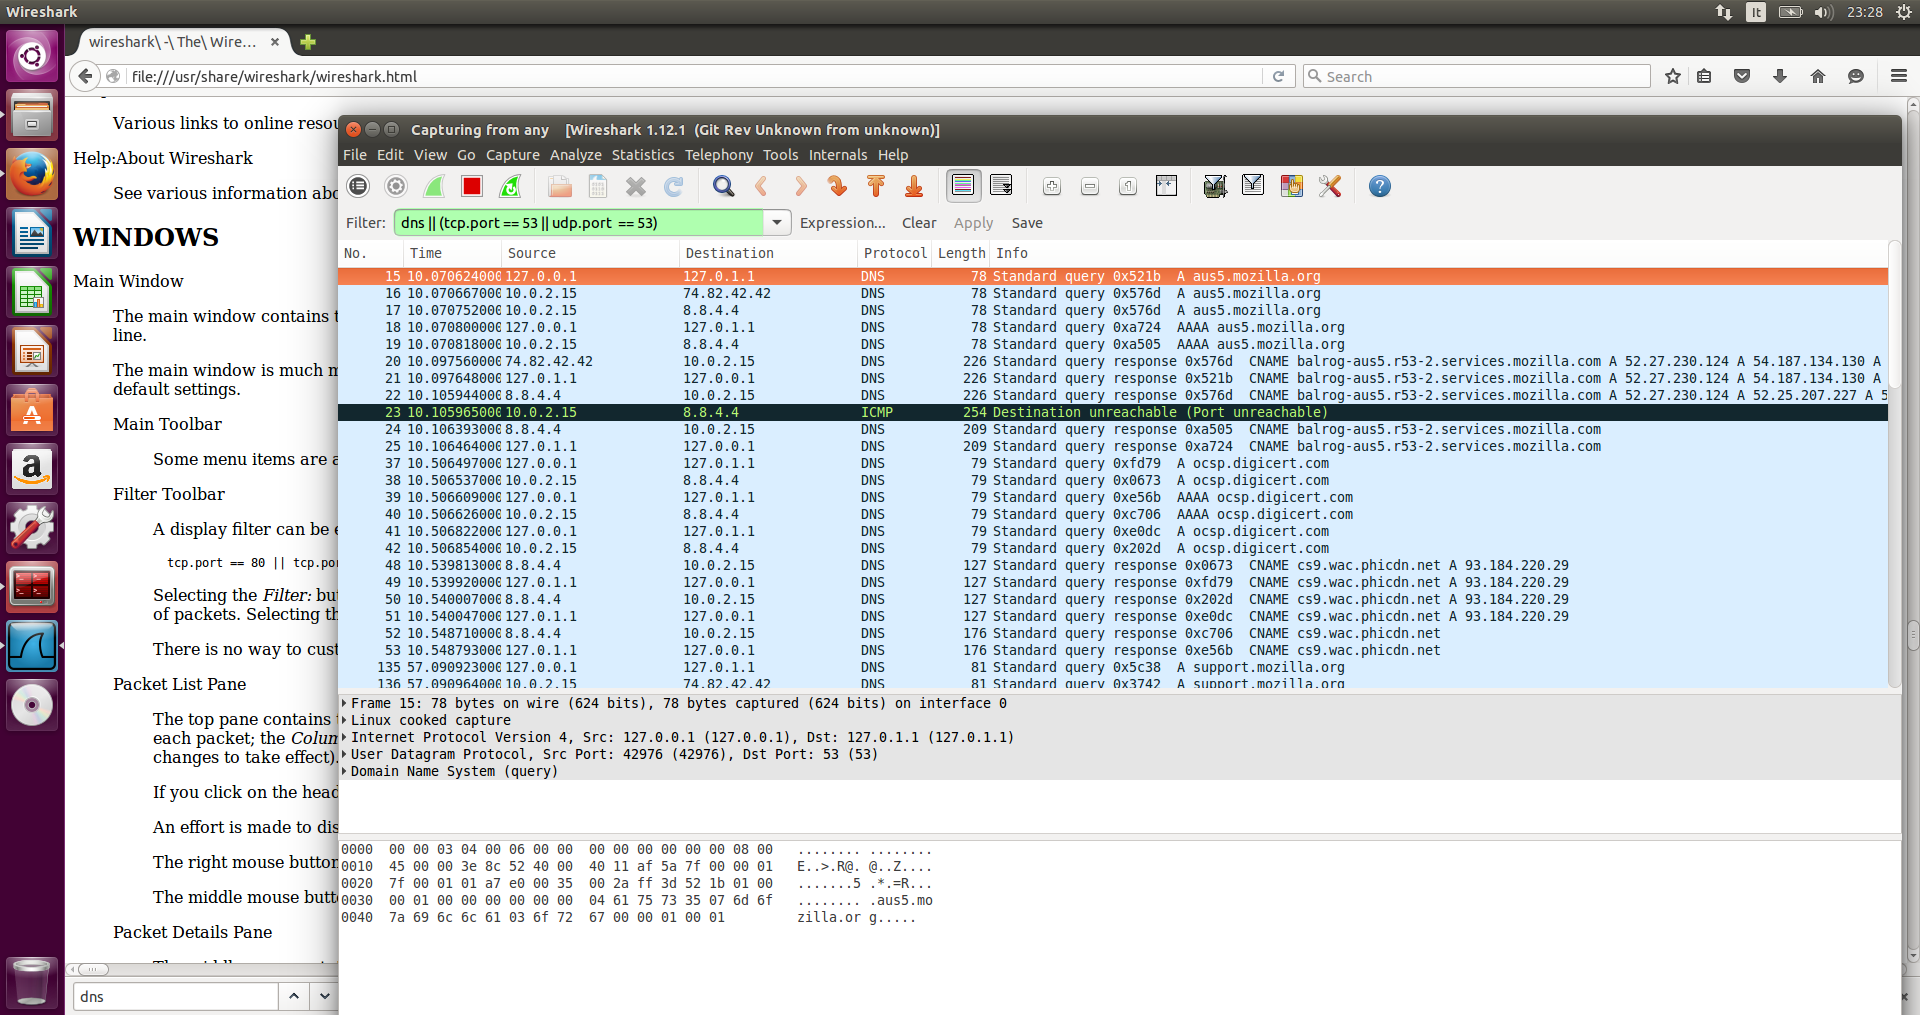
\includegraphics[width=0.9\textwidth]{img/lab2_1}}
\end{frame}

\section[Valutazione]{Valutazione}

\begin{frame}{Valutazione}{Formativa}
	\begin{block}{Risposta multipla -- Verifica delle conoscenze}
		\begin{enumerate}
			\item Con ``Domain Name System'' si intende:
			\begin{enumerate}[a]
				\item un sistema distribuito che \ldots
				\item \ldots
			\end{enumerate}
			
			\item Con indirizzo FQDN s'intende
			\begin{enumerate}[a]
				\item il nome completamente qualificato\ldots
				\item \ldots
			\end{enumerate}
			
			\item Gli svantaggi di un db centralizzato sono:
			\begin{enumerate}[a]
				\item singolo punto di guasto\ldots
				\item \ldots
			\end{enumerate}
			
		\end{enumerate}\hspace{0.45cm}$\vdots$

	\end{block}
\end{frame}

\begin{frame}{Valutazione}{Formativa}
	\begin{block}{Vero o falso }
		\begin{enumerate}
			\item Ad ogni host corrisponde un unico indirizzo IP?
			\item Un host pu\`o avere pi\`u nomi?
			\item Il DNS funziona solo in UDP?
			\item Il FQDN pu\`o essere arbitrariamente lungo?
		\end{enumerate}\hspace{0.45cm}$\vdots$

	\end{block}
\end{frame}

\begin{frame}{Valutazione}{Sommativa}
	\begin{block}{Relazioni sulle attivit\`a di laboratorio}
		Tutte le attivit\`a di laboratorio devono essere accompagnate da una relazione singola o in gruppo (BES) che deve essere caricata sulla piattaforma Moodle.
		
		La relazione \`e valutata secondo una griglia elaborata con gli studenti.
	\end{block}
	\begin{block}{Domande aperte -- orale o scritte}
			\begin{enumerate}
				\item Descrivi la procedura di risoluzione di un nome nel caso di interrogazione ricorsiva.
				\item Data la seguente configurazione di rete, indica la sequenza di request e response della query DNS \ldots{}
			\end{enumerate}
	\end{block}
\end{frame}

\begin{frame}[allowframebreaks]{Valutazione}{Sommativa}
	\begin{block}{Mini-progetto I}
Il Dirigente scolastico dell'Istituto d'Istruzione Superiore ``Edgser W. Dijkstra'' indice un bando per la progettazione e la realizzazione dell'infrastruttura di rete dell'Istituto.
Tale infrastruttura prevede la presenza di cinque reti locali connesse ad Internet: la rete del personale docente, quella del personale amministrativo, quella per i laboratori e, infine, una rete WiFi per i dispositivi degli studenti.

Alcuni host di ciascun dominio devono essere raggiungibili da Internet tramite host name (eventuali NAT sono a cura del docente), per garantire il funzionamento dei servizi di autenticazione, stampa, web, gestione dei dati\ldots{}.
	\end{block}
	
	\begin{block}{Mini-progetto II}
L'Istituto mette a disposizione un sistema per la simulazione della rete e delle macchine virtuali preconfigurato, cui i partecipanti al bando devono aggiungere \alert{i file di configurazione dei server DNS di competenza per ogni dominio e dei resolver degli host di ogni dominio}.
 
Si partecipi al bando inviando i file di configurazione e la relazione tecnica corredata dalla documentazione di progetto.

Ogni partecipante sar\`a valutato in base ai seguenti criteri: \ldots
	\end{block}

\end{frame}

\part[Colloquio]{Colloquio}

\begin{frame}[plain]
	
	\vfill
	
	\begin{center}
		{\Large GRAZIE PER L'ATTENZIONE!}
		
		\bigskip
		
		\begin{center}\Huge{Any questions?}\end{center}

	\end{center}
	
	\vfill
	
\end{frame}

\end{document}

\section[Deontologia insegnamento con il software]{Deontologia professionale nell'insegnamento con il software}

\begin{frame}[allowframebreaks]{Deontologia professionale e software per la didattica}{Perch� la scuola deve usare esclusivamente software libero}
	
	
	\textbf{Le istituzioni didattiche in genere, dalla scuola materna all'universit�, hanno il dovere morale di insegnare solo il software libero.} \hyperlink{http://www.gnu.org/education/edu-schools.it.html}{\beamerbutton{Articolo di R. Stallman}}
	
	\begin{block}{Estratti I}
		Il software libero consente alle scuole di risparmiare, anche se questo � un beneficio secondario {[}\ldots{]}
		\medbreak
		La scuola ha una missione sociale: insegnare a chi studia a diventare cittadino di una societ� {[}\ldots{]} collaborativa e libera.
		\medbreak
		Al contrario, insegnare un programma non libero crea dipendenza, e questo va contro la missione sociale delle scuole: le scuole non dovrebbero mai farlo.
	\end{block}
	
	\begin{block}{Estratti II}
		\medbreak
		Il software libero consente a chi studia di poter imparare il funzionamento di un programma.
		\medbreak
		Il software libero incoraggia tutti ad imparare.
		\medbreak	
		Come si impara a scrivere codice per programmi complessi? Scrivendo tante piccole modifiche per programmi complessi esistenti. Il software libero lo permette, il software proprietario lo vieta.
		\medbreak	
		La pi� profonda motivazione in sostegno all'utilizzo del software libero nella scuola � per la formazione morale.
		\medbreak	
		Insegnare a chi studia l'uso del software libero, e a far parte della comunit� del software libero, � una lezione di educazione civica sul campo.
	\end{block}
\end{frame}

